\documentclass[11pt, a4paper]{article}

\usepackage{amsmath}
\usepackage{amssymb}
\usepackage{graphicx}
\usepackage{listings}
\usepackage{color}
\usepackage[section]{placeins}
\usepackage{paralist}
\usepackage{fullpage}
\usepackage{glossaries}

\usepackage{caption}
\usepackage{subcaption}

\newacronym{DNS}{DNS}{Domain Name System}

\newcommand*{\titleGM}{\begingroup
\hbox{ 
\hspace*{0.2\textwidth} 
\rule{1pt}{\textheight} 
\hspace*{0.05\textwidth} 
\parbox[b]{0.75\textwidth}{ 

{\noindent\Huge\bfseries Rapid Growth in Top Level Domains in the Domain Name System}\\[2\baselineskip] % Title
{\large \textit{SEM5720 - Assignment 1}}\\[4\baselineskip] % Tagline or further description
{\Large \textsc{Alexander D Brown (adb9)}} % Author name

\vspace{0.5\textheight} 
}}
\endgroup}


\begin{document}
\titleGM 
\tableofcontents
\newpage

\section{Introduction}
% - Introduce domain names
Domain names map a humanly memorable host name to a less memorable machine IP
address used to route traffic to that host. \gls{DNS} is a distributed database
made up of name servers and provides a mapping from domain name to IP address 
and vice versa.

The lookup process is recursive by nature as the name servers are laid out in a
tree structure, starting from an unnamed root, each layer of the tree 
represents each part of the domain name.

\begin{figure}[h]
\centering
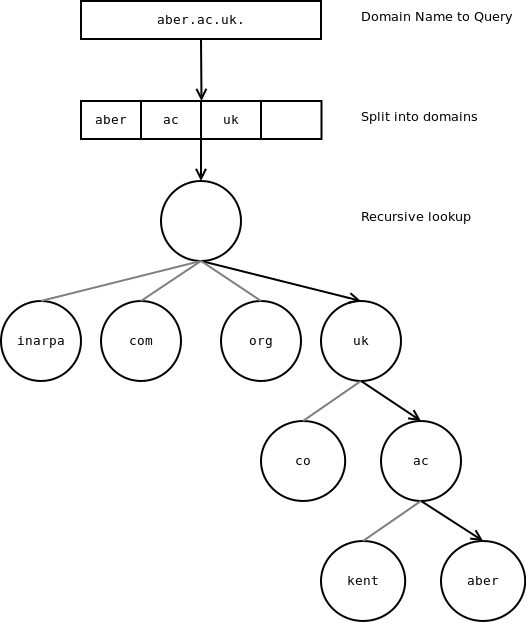
\includegraphics[width=0.5\textwidth]{img/dns-lookup}
\caption{Example DNS Lookup on \texttt{aber.ac.uk.}}
\end{figure}

% - Introduce the Domain Name System
%   - Explain top level domains


\nocite{Manning2011Challenges}
\nocite{rfc3226}

\newpage
\bibliographystyle{plain}
\bibliography{citations}

\end{document}
